\documentclass[journal]{IEEEtran}

\def\P(#1){\Phelper#1|\relax\Pchoice(#1)}
\def\Phelper#1|#2\relax{\ifx\relax#2\relax\def\Pchoice{\Pone}\else\def\Pchoice{\Ptwo}\fi}
\def\Pone(#1){\Pr\left( #1 \right)}
\def\Ptwo(#1|#2){\Pr\left( #1 \mid #2 \right)}
\def\Pr{\mathbf{Pr}}

\usepackage[utf8]{inputenc}
\usepackage{graphicx}
\usepackage{amsmath}
\usepackage{amsthm}
\usepackage{amssymb}
\usepackage{hyperref}
\usepackage{subfig}
\usepackage{multirow}
\usepackage[section]{placeins}

\usepackage{tabularx,booktabs}
\newcolumntype{C}{>{\centering\arraybackslash}X} % centered version of "X" type
\setlength{\extrarowheight}{1pt}
\usepackage{lipsum}
\usepackage[table]{xcolor}


\renewcommand\thesection{\arabic{section}}


% correct bad hyphenation here
\hyphenation{op-tical net-works semi-conduc-tor}


\begin{document}
\title{Multi-Object Target Disappearance Prediction }
\author{Akanksha~Dwivedi(MT2016006)
        and~Tarini~Chandrashekhar(MT2016144),~\IEEEmembership{International Institute of Information Technology, Bangalore}}% <-this % stops a space

% The paper headers
\markboth{Machine Learning Project Report, \today}%
{Shell \MakeLowercase{\textit{et al.}}: Bare Demo of IEEEtran.cls for IEEE Journals}

\IEEEspecialpapernotice{(Draft Paper)}

% make the title area
\maketitle

% As a general rule, do not put math, special symbols or citations
% in the abstract or keywords.
\begin{abstract}
We present a novel approach to detect whether an object is going to be remain in the next frame, or not, given its previous trajectory, and relative location with respect to the entire frame. Given the dataset containing the bounding box coordinates and the ground truth values of the objects in the frames, design a network which learns these values to generate a trajectory for each object, where each object would have multiple sequences in which it would appear and subsequently disappear, either exiting naturally, or getting occluded by another object. The network learns this by multiple sequences and as a result, given a frame, can classify whether the object will remain in the next frame or not.
\end{abstract}

% Note that keywords are not normally used for peer review papers.
\begin{IEEEkeywords}
sequences, Inception, Tensorflow, GRU, LSTM.
\end{IEEEkeywords}
   
\IEEEpeerreviewmaketitle

\section{Introduction}
Tracking of multiple targets in uncontrained environments is a challenging task, and is still far from reaching the accuracy of human labelling. A major part of tracking is keeping track of objects going out of frame, when they exit or get occluded by another object. There is little work done in this area, even with the recent rise of deep learning. With this knowledge of next frame, given its history, the problem of data association can be made easier. In order to know the state of the next frame, we need long-term memory, and for this purpose, we use a simpler form of Long-Short-Term-Memory(LSTM) networks, called Gated Recurrent Unit(GRU). Our main work is as follows:

\begin{itemize}
    \item We present a form of Recurrent Neural network, which perform the work of generating a form of trajectory for each object based on its history.
    \item We use the optical quality of the objects as well their location with respect to the frame to get a consolidated feature, which is then fed into the recurrent network.
    \item The trajectory generated by the recurrent network in then fed to a fully connected layer,which then predicts about the presence of the object in the next frame.
    
\end{itemize}
The MOT2015 Dataset consists of 22 video sequences, partitioned equally in training and testing sets. Each video sequence folder consists of the following three folders:
    \begin{itemize}
        \item det: This contains the detection coordinates of the objects.
        \item gt: This contains the ground truth coordinates of the objects.
        \item img1: This contains the frames into the said video is broken into. The frames vary for videos vary from 7-30 FPS.
    \end{itemize}
All images were converted to JPEG and named sequentially to a 6-digit file name (e.g. 000001.jpg). Detection and annotation files are simple comma-separated value (CSV) files. Each line represents one object instance, and it contains 10 values. 
\par
The following table describes the values in the det and gt files:
\begin{figure}[ht!]
    \centering
    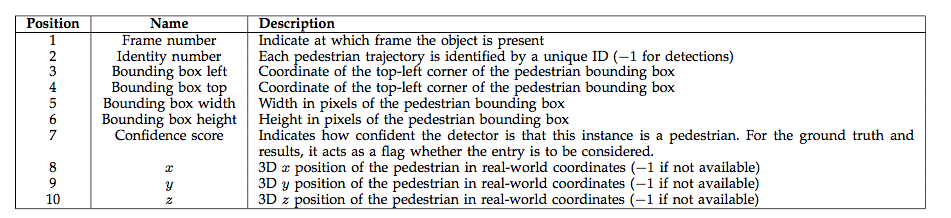
\includegraphics[scale = 0.3]{Dataset.png}
    \caption{Data format for the input and output files, both for detection and annotation files.}
    \label{fig:data}
\end{figure}


\section{Related Work}
In tracking-by-detection, a major challenge of online Multi-Object tracking is to how robustly associate noisy object detections on a new video frame with previously tracked objects.[1] formulate the online MOT problem as decision making in Markov Decision Process (MDPs), where the lifetime of an object is modeled with an MDP. They learn the similarity function for data association by learning a policy for MDP and policy learning is approached in a reinforcement learning fashion, benefiting from both offline-learning and online-learning for data association. Tracking multiple objects in real-world scenes involves many challenges including a) an a-priori unknown and time varying number of targets b) a continuous state estimation of all present targets, and c) a discrete combinatorial problem of data association. [2] propose an end-to-end deep learning approach for online multi-target tracking, by using recurrent neural networks. Inspired by the Bayesian filtering idea, they present a recurrent neural network capable of performing all multi-target tracking tasks including prediction, data association, state update as well as initiation and termination of targets within their unified architecture. They also present a way to generate arbitrary amounts of training data by sampling from a generative model. This was the first approach introducing the idea of recurrent neural networks to address the problem of online multi-target tracking. The performance achieved by the former was not very significant but recommends to incorporate appearance based features and learning through more robust association strategy.

\section{Proposed Work}
The diagram below briefly describes the architecture of the proposed network.
\begin{figure}[ht!]
    \centering
    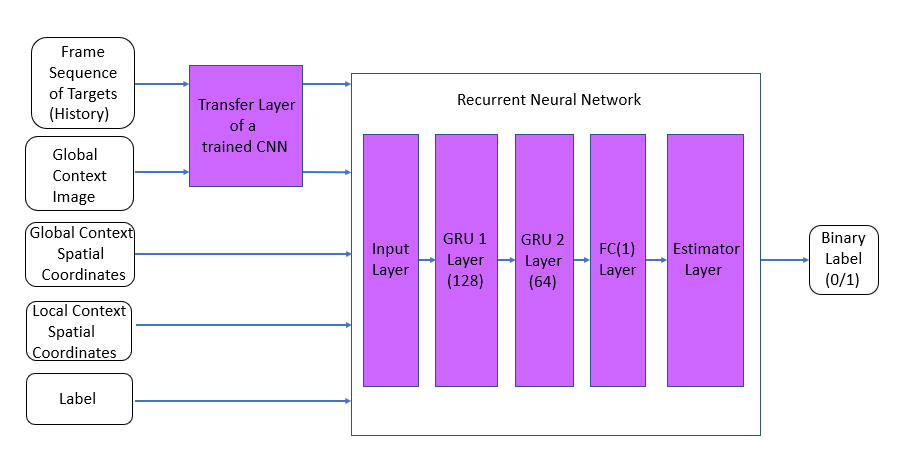
\includegraphics[width=9cm, height=5cm]{model_arch.PNG}
    \caption{Proposed Network Architecture}
    \label{fig:model_arch}
\end{figure}
\newline
Our architecture consists of the two major modules:
\begin{itemize}
    \item \textbf{Convolutional Neural Network} - We use a pre-trained CNN model, Inception v4, in order to get the feature vectors from the MOT Dataset 2015.
    \item \textbf{Recurrent Neural Network} -  We use a Gated Recurrent Unit(GRU), a type of RNN, to train the features we get from the CNN, along with location information from local and global context, and feed the result to a fully connected layer, followed by a softmax layer, to make a prediction at the end.
\end{itemize}

\subsection{Convolutional Neural Network}
We use a pre-trained model, Inception v4, and get the output from its last but one layer, the pool layer, to get feature vectors for our frames as well as for the cropped images of individual objects. The last layer of Inception model performs Image classification(for around 2000 classes of objects), but for our purposes, we need feature vectors of local and global context of the frame, so we just extract the output out of the pool layer and append it to our features, and then append the location information, i.e. frame dimensions and the bounding box dimensions for each object, Then it gets passed on to the next module of the architecture, the GRU.


\subsection{Recurrent Neural Network}

\subsubsection{Input layer}
The feature vector for each frame consists of four components - 1.Convoluted feature vector of the entire frame, 2. Convoluted feature vector of just an object, i.e feature vector of the object, cropped out of the original frame according to its bounding box dimensions, 3.Pixel dimensions of the frame, and 4.Bounding box dimensions of the object,i.e. [x,y,x+w,y+h]. Now, we need to be careful about the fact that we need to make the network learn the trend of the object exiting/disappearing the frame. So, we extract, for each object, contiguous sequences at the end of which the object disappears. So, each of these sequences is a data point. So, we train sequences. As for labels, for each sequence, we take a fixed value called historyLength, which is the number of time steps we look back, to determine the prediction. Now, we take 'k' such random subsets out of the sequence, of length historyLength. $\frac{1}{k^{th}}$ subset, is given the label 1, and the rest of them are given the label 0. Label 0 means the object remains in the next frame, and 1 means the object disappears in the next frame. Since there are contiguous sequences of varying lenghts throughout the videos, this method helps us retain a uniform length datapoint and label, one which can be fed into the model. We would do well to keep a check on the size of the sequence, i.e take the sequences which are marginally longer than the historyLength, in order to get different subsets of historylength, which are unrepetitive. We split the features and labels into training and testing data.

After this, we create the network using tflearn library, where we feed the input tensor of shape, historyLength x InputDimSize, where InputDimSize = 4104( 2048+2048+4+4).

\subsubsection{GRU layers}
We employ two hidden GRU layers - the first layer layer with 128 units and returns a sequence, which is then fed into the second GRU layer, which consists of 64 units.

\subsubsection{Fully Connected Layers}
We apply a softmax function to  "squash" a K-dimensional vector  of arbitrary real values to a K-dimensional vector of real values in the range [0, 1] that add up to 1. The finally computation of the neural network is performed in this layer. To avoid overfitting, we apply L2-regularization. 

\subsubsection{Estimator Layer}
This is basically a regressor layer. The final layer of this network is optimized using Adam optimizer, which inherits from Rmsprop and AdaGrad optimizers. Some of its features are that parameters updates are invariant to re-scaling of gradient. It means that if we have some objective function f(x) and we change it to k*f(x) (where k is some constant). There will be no effect on performance. Secondly, it doesn’t require stationary objective. That means the f(x) might change with time and still the algorithm will converge. Adam is scale invariant. We calculate the mean-square loss function and perform regression to predict labels for test data, giving a learning rate of 0.001-0.002. 


\section{Results}
We ran the model for five epochs and got a testing accuracy ranging between 73-77$\%$. The least loss and maximum accuracy was incurred with loss function as mean-square and with Adam Optimizer. The Stochastic Gradient Descent(SGD) as an optimizer incurred the maximum error while training. We got a maximum training accuracy of 77$\%$. The screenshot below shows the accuracy and loss encountered while training the network.

\begin{figure}[ht!]
    \centering
    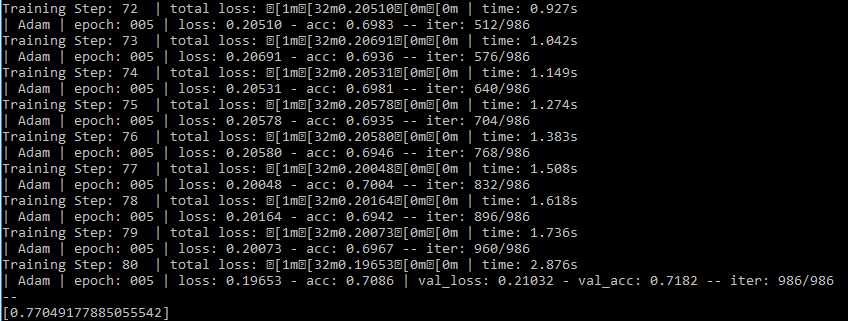
\includegraphics[scale = 0.35]{run.PNG}
    \caption{Screenshot of running the network}
    \label{fig:run}
\end{figure}

We kept 90$\%$ of the data as training set and the rest as testing set. Further, 10$\%$ of the training data was used as validation set. In the prediction figure below, we compared the labels predicted by the model with the ground truth labels. The green xs represent the predicted labels while the red dashes represent the ground truth.
\newline
Following the prediction figure, the figures with training and testing accuracy and the training and validation loss with tuned hyperparameters are shown.

\begin{figure}[ht!]
    \centering
    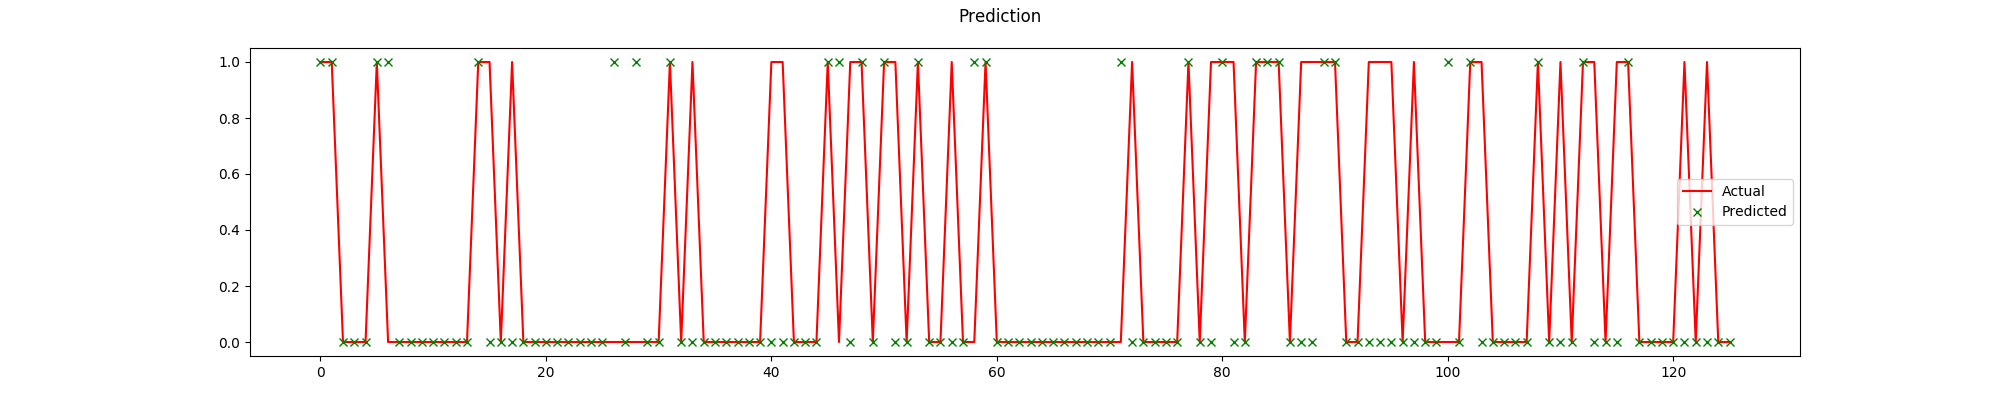
\includegraphics[width=10cm, height=2.8cm]{Prediction.png}
    \caption{Comparison of final predicted labels by the network with ground truth}
    \label{fig:Prediction}
\end{figure}

\begin{figure}[ht!]
    \centering
    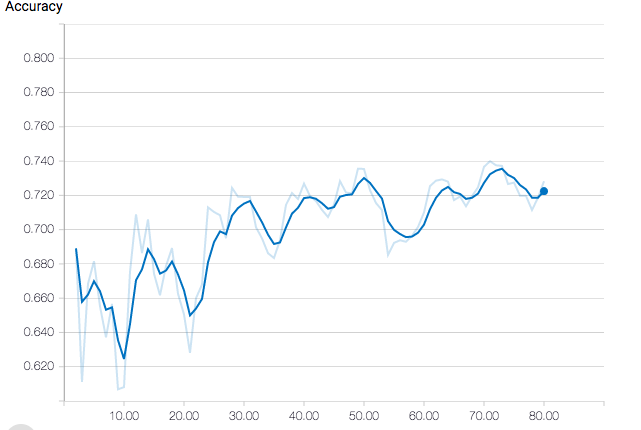
\includegraphics[scale = 0.3]{Acc_76_1.png}
    \caption{Overall Accuracy of the network}
    \label{fig:Acc1}
\end{figure}

\begin{figure}[ht!]
    \centering
    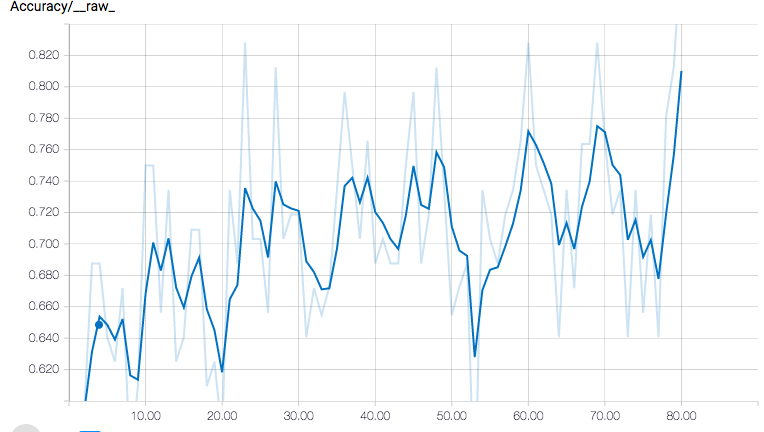
\includegraphics[scale = 0.3]{Acc_76_2.png}
    \caption{Training accuracy of the network}
    \label{fig:Acc2}
\end{figure}

\begin{figure}[ht!]
    \centering
    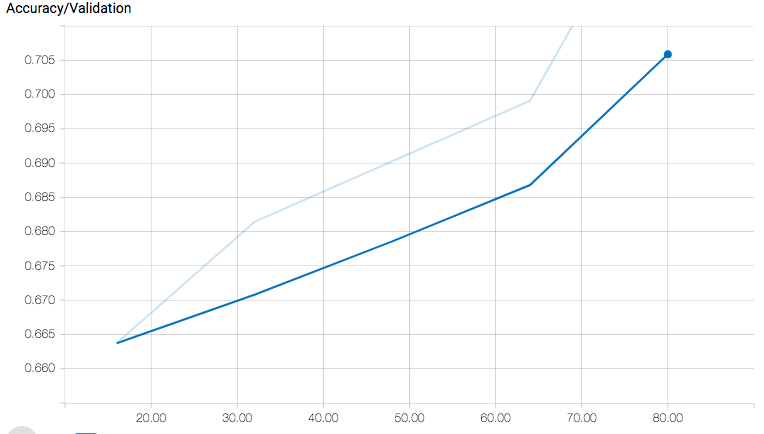
\includegraphics[scale = 0.3]{Acc_76_3.png}
    \caption{Validation Accuracy of the network}
    \label{fig:Acc3}
\end{figure}

\begin{figure}[ht!]
    \centering
    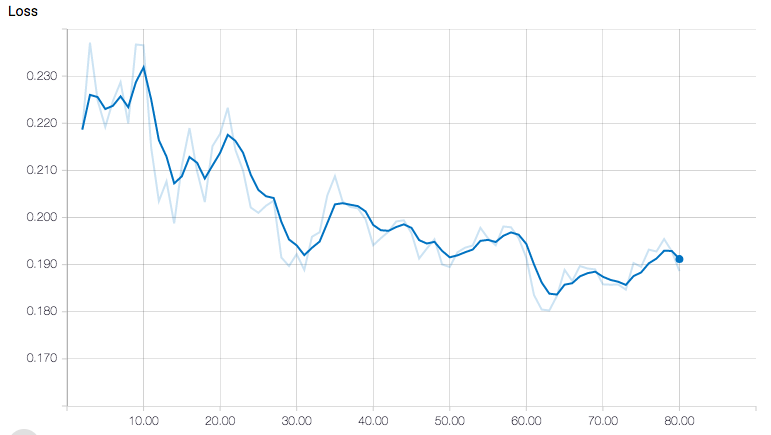
\includegraphics[scale = 0.3]{Acc_76_4.png}
    \caption{Overall loss incurred by the network}
    \label{fig:loss1}
\end{figure}

\begin{figure}[ht!]
    \centering
    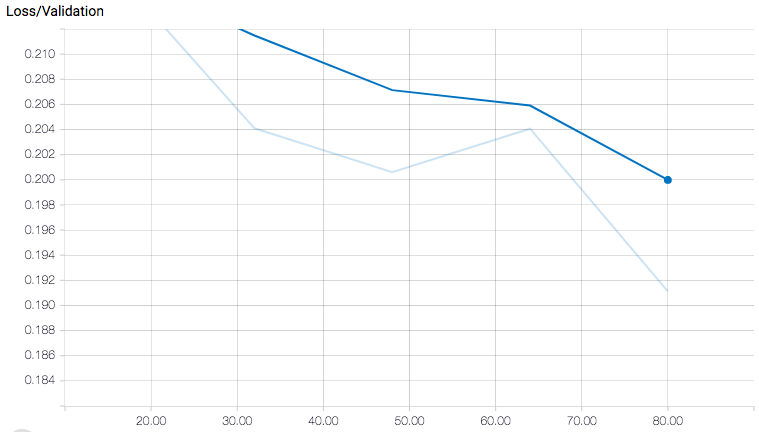
\includegraphics[scale = 0.3]{Acc_76_5.png}
    \caption{Loss incurred by the network during validation}
    \label{fig:loss2}
\end{figure}
While the 5 figures capture the summary for the best model learnt, the last two figures presents the relative accuracy achieved and loss occured among multiple variants of the network (i.e. learnt by changing the hyperparameters of the model)
\begin{figure}[ht!]
    \centering
    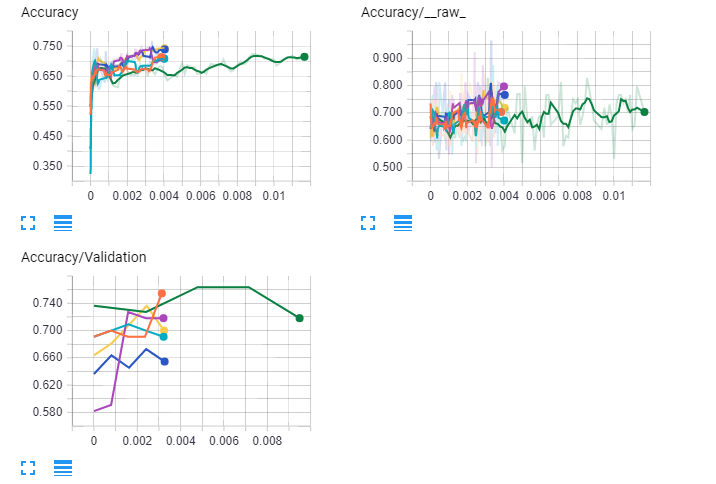
\includegraphics[scale = 0.4]{rel_all_acc.PNG}
    \caption{Relative Training and Validation Accuracy of all models}
    \label{fig:rel_acc}
\end{figure}

\begin{figure}[ht!]
    \centering
    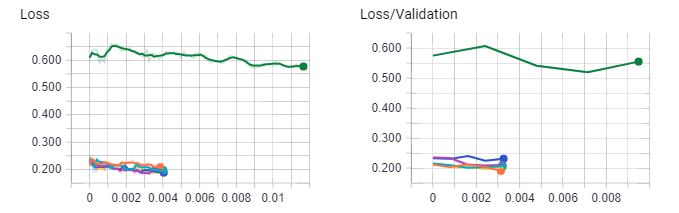
\includegraphics[scale = 0.45]{rel_all_loss.PNG}
    \caption{Relative Loss incurred by all models}
    \label{fig:rel_loss}
\end{figure}


\section{Conclusion}
Looking at the above graphs and predictions, we concluded, that while predictions were unbiased, the proportion of 1's in the labels were less as compared to the 0's, i.e the object appears more frequently than it disappears, naturally. So, there are chances, if we keep too high a value of 'k'(ratio of number of 1's to 0's in labels), the dataset might become skewed, containing proportionally more 0's than 1's. It will give a better accuracy, but with a biased dataset. So, it will do well to choose the value of 'k' carefully. We can see from the graphs that with each training step, the training accuracy and the validation accuracy increases and the training loss and validation loss decreases. As tested with trial and error, we get the best results with mean square loss function.

\section{Future Work $\&$ Improvements}
Our proposed architecture is an attempt to model the target's disappearance/death in a Multi-Object-Tracking problem using recurrent neural networks. Recurrent neural networks successfully capture the long term dependencies in a sequence, which is particularly useful in the object tracking problem. However, our proposed network only covers a small part of MOT problem i.e. estimating whether the target appears in the frame or has gone out of the frame, using its modeled history.
\begin{itemize}
    \item The next step would be to perform data association task i.e. associating the detections in multiple frames in a sequence for each target, to identify both birth/death of targets in the sequences.
    \item The final phase of the problem statement would consist of tracking multiple targets in a video sequence using the data associations.
    \item We extracted the features from the second to last layer of already trained Inception-v4 model. However the dimension of features was limited to 2048 and the model is trained for a large number of different classes. Another custom convolutional network can be trained from scratch, only on the human data, to provide more sophisticated and high dimensional features.
    \item A more wider/deeper model can be built by adding more hidden units/layers in the recurrent neural network.
    \item Due to memory constraints, we made an assumption of only considering the 10 recent frames as the historyLength of the target. This number can be increased by simultaneously balancing the the ratio of 0 and 1 label samples to avoid skewness in the dataset.
    \item Dynamic length sequences can be accommodated by using padding in the sequences, before feeding the input to the network.
    \item We ignored the sequences which have significantly less number of frames. In future works, they could be highlighted to the model as false positives and reinforced in a way, to avoid similar failures. 
    \item As we used features of a sequence as a single datapoint, the data got reduced after final pre-processing of data. More data needs to be considered, to increase the accuracy of the model, with significant amount of hardware.
\end{itemize}

\section*{Acknowledgment}
We would like to extend our gratitude to our instructor, Prof. G. Srinivasaraghavan, whose invaluable guidance helped us build our intuition and gave our work a more academic perspective.


\ifCLASSOPTIONcaptionsoff
  \newpage
\fi

\section{Data $\&$ Code}
\begin{itemize}
    \item Data : \url{https://motchallenge.net/data/2D_MOT_2015/} 
    \item Code : \url{https://github.com/tarini92/Project-Elective-II}
\end{itemize}

\begin{thebibliography}{1}
\bibitem{LearningToTrack}
Yu Xiang, Alexandre Alahi and Silvio Savarese.
\textit{Learning to Track: Online Multi-Object Tracking by Decision Making}
\bibitem{onlineMOT} 
Anton Milan, S. Hamid Rezatofighi, Anthony Dick, Ian Reid and Konrad Schindler. 
\textit{Online Multi-Target Tracking Using Recurrent Neural Networks}.
\bibitem{humanTrajectoryPrediction}
Daksh Varshaneya, Prof. G. Srinivasaraghavan
\textit{Human Trajectory Prediction using Spatially aware Deep Attention Models}
\bibitem{Inception}
\textit{Inception-v4}
\url{https://arxiv.org/abs/1602.07261}
\bibitem{TFLearn}
\url{http://tflearn.org/getting_started/}

\end{thebibliography}



\end{document}